\documentclass[12pt,tikz]{standalone}

\usepackage{graphicx}
\usetikzlibrary{positioning}
\begin{document}

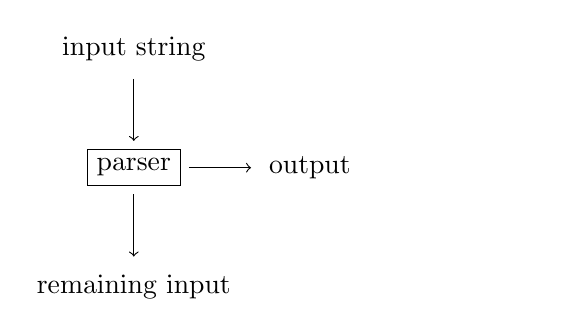
\begin{tikzpicture}[draw, ->, black, shorten >=3pt, shorten <=3pt, node distance = 1cm]
  \node at (10, 0) (dummy) {};

  \node at (5, 0) (input) {input string};
  \node[below = of input, draw, rectangle] (parser) {parser};
  \node[right = of parser] (output) {output};
  \node[below = of parser] (rest) {remaining input};

  \draw (input) -- (parser);
  \draw (parser) -- (output);
  \draw (parser) -- (rest);
\end{tikzpicture}

\end{document}
